\documentclass{standalone}
\usepackage[dvipsnames,svgnames,x11names]{xcolor}
\usepackage{tikz}
\usepackage{pgfplots}
\pgfplotsset{compat = 1.12}
\usepackage{../thesismath}
\begin{document}
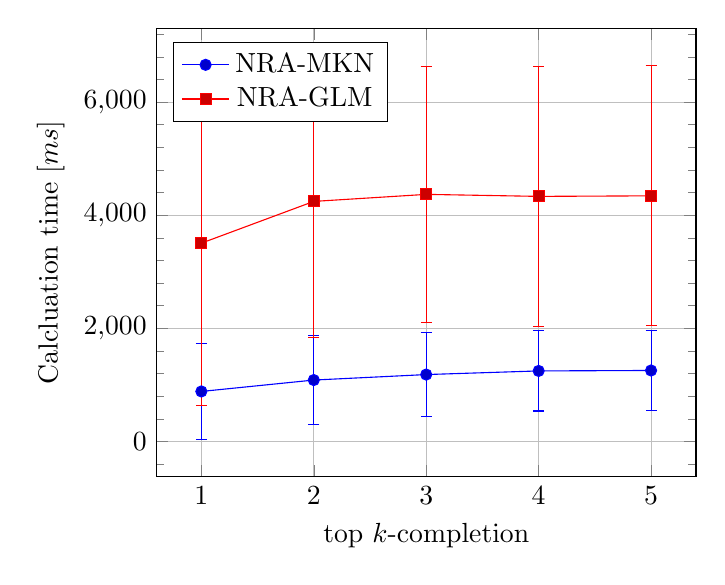
\begin{tikzpicture}[baseline]

\begin{axis}[
  xlabel = {top $k$-completion},
  xtick = {1, ..., 5},
  ylabel = {Calcluation time [$m s$]},
  minor y tick num = 4,
  grid = major,
  legend entries = {{NRA-MKN}, {NRA-GLM}},
  legend pos = north west,
]

% over 100 test sequences on my own machine

% NRA-MKN
\addplot+[
  error bars/.cd,
  y dir = both,
  y explicit,
] table [y error = us_error] {
  n us       us_error
  1  883.680  844.083
  2 1085.228  787.949
  3 1182.359  746.578
  4 1246.696  708.485
  5 1254.554  707.658
};

% NRA-GLM
\addplot+[
  error bars/.cd,
  y dir = both,
  y explicit,
] table [y error = us_error] {
  n us       us_error
  1 3506.086 2871.907
  2 4244.655 2402.179
  3 4369.192 2266.325
  4 4333.634 2297.886
  5 4343.249 2300.984
};

\end{axis}

\end{tikzpicture}
\end{document}
